\section{Pickup}
\label{pickup}

Electric guitars pickups are usually built by wrapping copper wire around magnets.
The working principle is based on the variation of magnetic field, created by the string
vibration. The vibration frequency of the string induces an electric signal on the output of the pickup
\cite{pickup-work, faraday-law}.

The designed pickup used the following main components:

\begin{itemize}
  \item Base to assembly the set up magnet+coil
  \item 6 magnets
  \item Copper wire to wrap the magnets
  \item Cover to attach the set up on the guitar
\end{itemize}

After some studies it was decided to build the pickup base using a 3D printer, due the
availability and reduced cost of this project. The model is showed on \autoref{3D-project}
and was projected using the AutoCAD software.

\begin{figure}[!htpb]
\centering
\caption{3D pickup base project}
\label{3D-project}
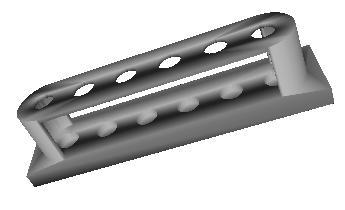
\includegraphics[scale=0.5]{images/pickup}
\legend{Source: Authors}
\end{figure}

There were two materials available to print the model, \textit{PLA} (Polylactic Acid)
and \textit{ABS} (Acrylonitrile Butadiene Styrene) \cite{3d-materials}. It was decided to print
the model on PLA because it attends the requisites of robustness of the project, is
faster to print and have a lower cost when compared to the other materials. The built part is showed on
\autoref{3D-base}

\begin{figure}[!htpb]
\centering
\caption{3D pickup base, TODO: take better picture}
\label{3D-base}
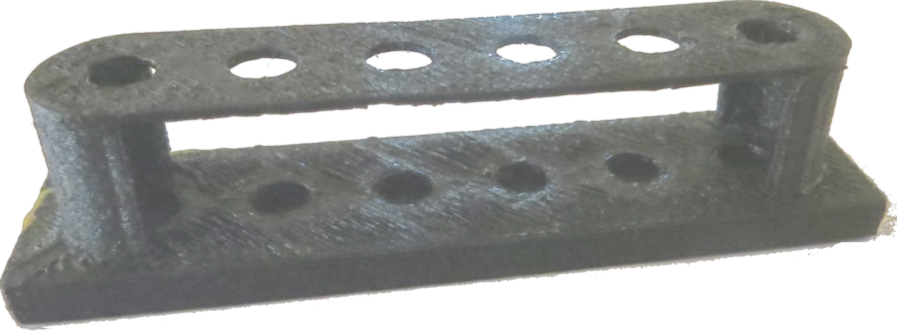
\includegraphics[scale=0.08]{images/base}
\legend{Source: Authors}
\end{figure}

With the pickup base ready, the coils were dimensioned. The area of a turn
was considered as a square with side dimensions equal to the wire diameter, and using that
it was estimated the wire diameter as in \autoref{wire-diameter-equation}.

\begin{equation}
  \label{turns-equation}
  Turns = \frac{Area\ between\ magnets}{Area\ of\ each\ turn} = \frac{ w * l / 2 }{ d^{2} } = \frac{5 mm * 12 mm / 2}{d^2} = 1000
\end{equation}
\begin{equation}
  \label{wire-diameter-equation}
  d = \sqrt{\frac{w\ *\ l}{2\ *\ Turns}} = \sqrt{\frac{5 mm * 12 mm}{2*1000}} \cong 0.17 mm \cong 34 AWG
\end{equation}

\autoref{turns-equation} was used with 1000 turns as a reference, based on a similar project
\cite{hexaphonic-pickup}. Using the area between 2 magnets (5 mm wide
and 12 mm length) and the estimated area of a wire turn it is possible to calculate the wire diameter,
as in \autoref{wire-diameter-equation} - resulting in a diameter of 0.17 mm, that can be
converted to 34 AWG, approximately. 

This diameter (number of turns) is only feasible with an automated process. The present project was built by manually
wrapping copper wire around each magnet (\autoref{magnets}), so only 500 turns were feasible. 

After mounting the coils, as showed on \autoref{coils} it was performed a test to verify the real voltage value induced by
the variation of the magnetic field. It was used the LM 741 \cite{LM741} with a gain of 10,
because it wasn't possible to verify the value on the coil output. With this simple test circuit
it was possible to verify that the output value on the IC was 8 mV, this value indicate that the
output value on the coil is around 1 mV.

\begin{figure}[!htpb]
  \centering
  \caption{Magnets used on the project}
  \label{magnets}
  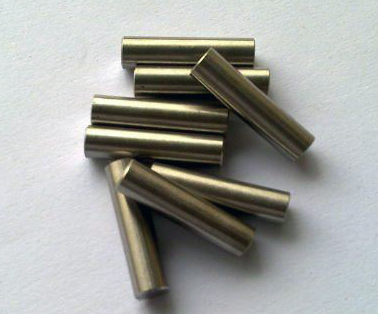
\includegraphics[scale=0.3]{images/magnets}
  \legend{Source: \citeonline{pickup-magnets}}
\end{figure}

\begin{figure}[!htpb]
  \centering
  \caption{Coils assembled}
  \label{coils}
  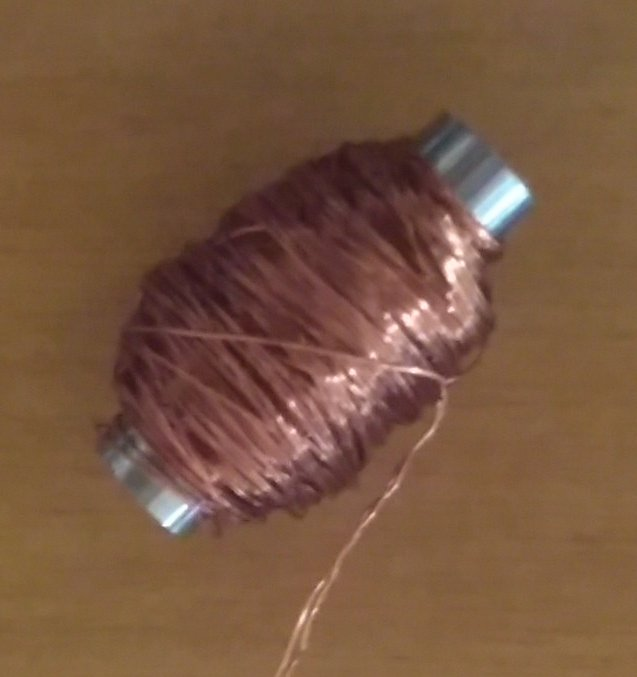
\includegraphics[scale=0.08]{images/coils}
  \legend{Source: Authors}
\end{figure}

After testing with one coil, the complete assemble was made, as showed on \autoref{6coils}
and \autoref{assembled-pickup}.

\begin{figure}[!htpb]
  \centering
  \caption{Coils assembled}
  \label{6coils}
  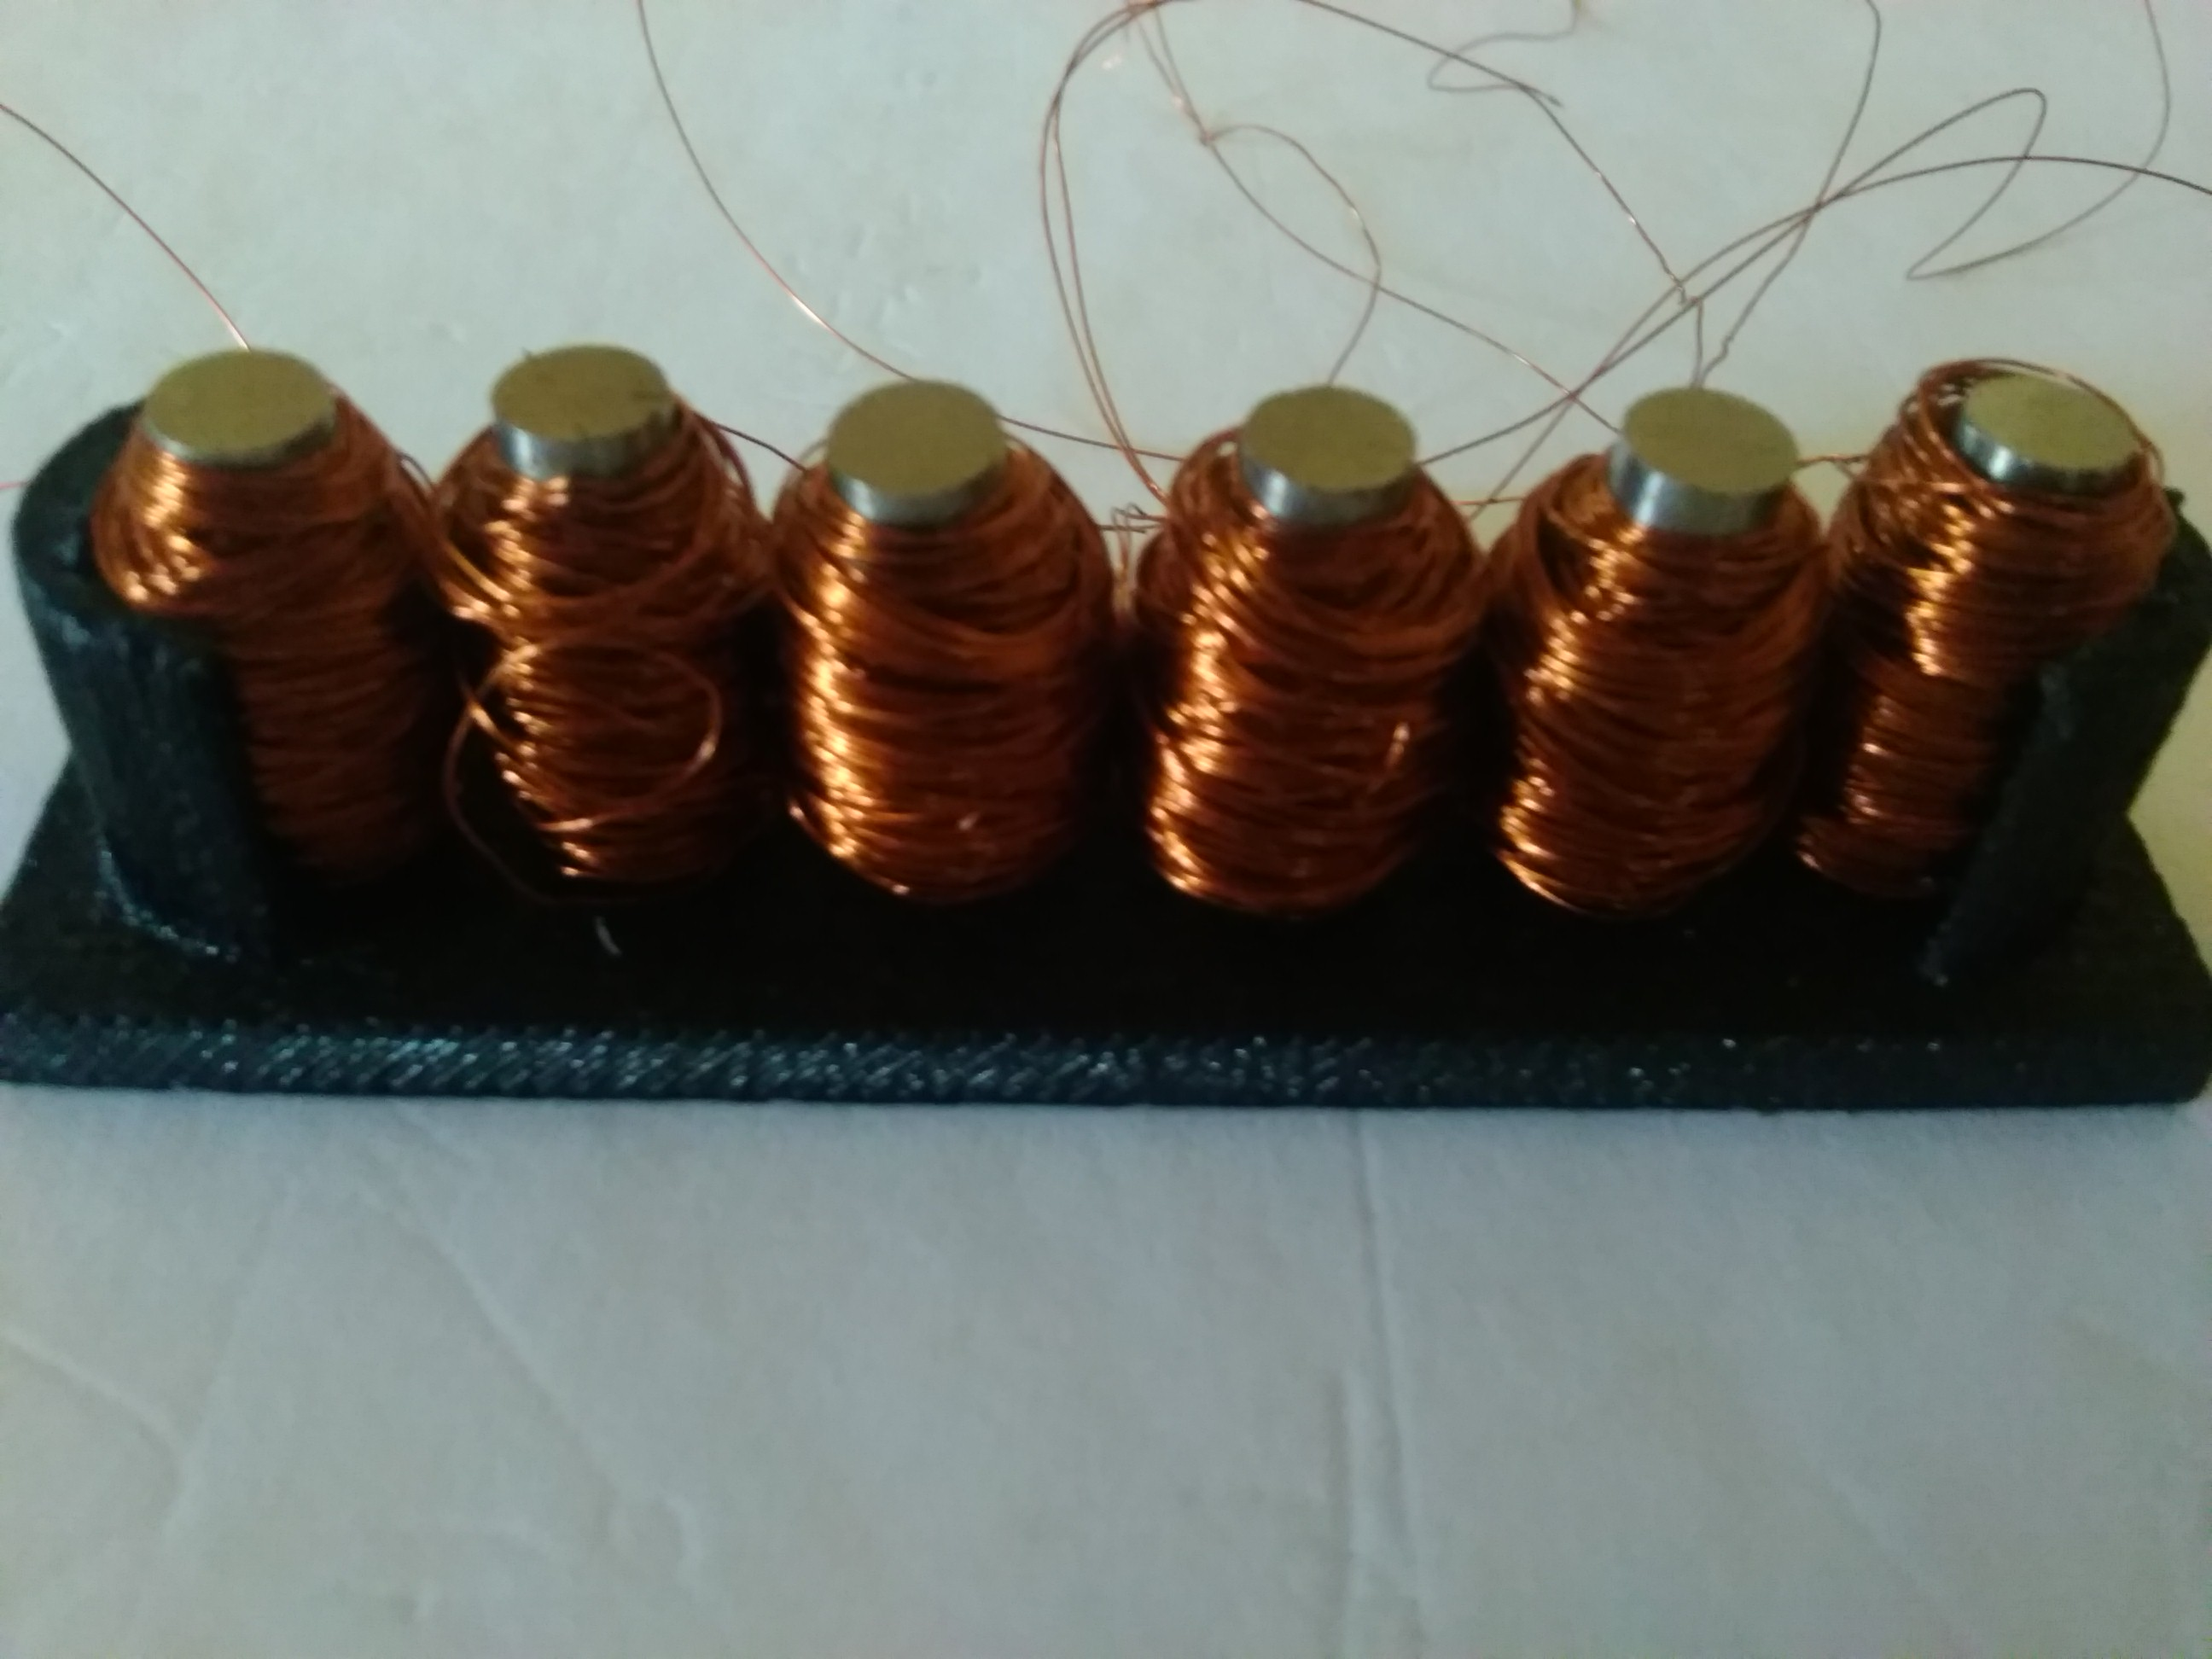
\includegraphics[scale=0.08]{images/6coils}
  \legend{Source: Authors}
\end{figure}

\begin{figure}[!htpb]
  \centering
  \caption{Coils assembled}
  \label{assembled-pickup}
  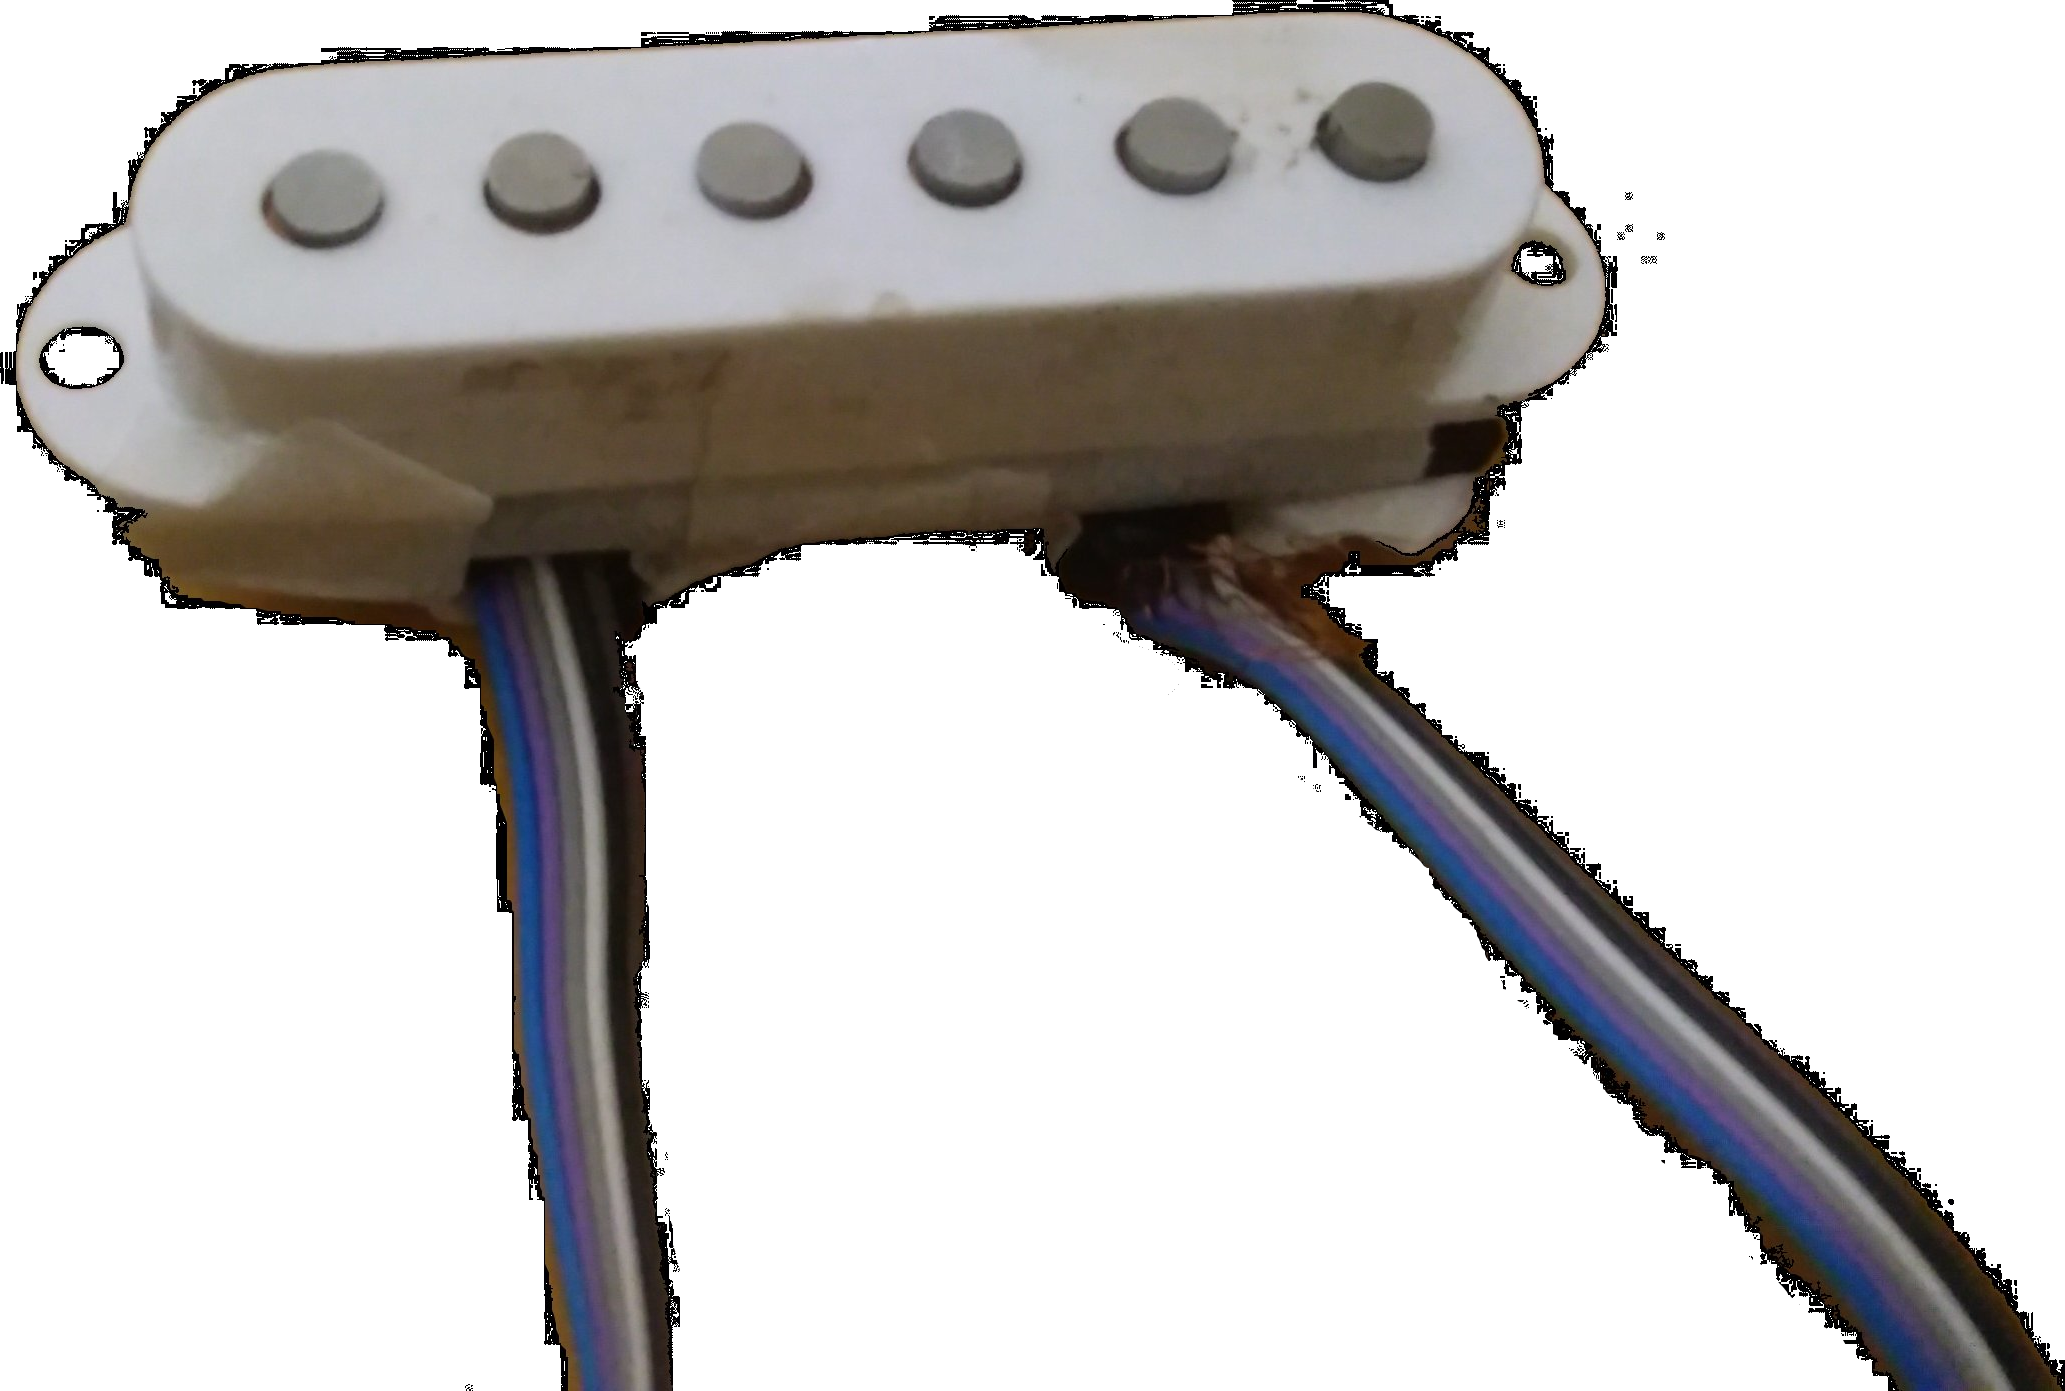
\includegraphics[scale=0.08]{images/assembled-pickup}
  \legend{Source: Authors}
\end{figure}
